\newlength{\bibsep}
\documentclass[nonatbib,1p,a4paper,12pt]{elsarticle}  % 5p for two columns, 1p for 1 column (this is specific for the elsearticle)
\usepackage[english,norsk,nynorsk]{babel}        % Language
\usepackage[DatePublished]{Code/NTNU-lab}        % remove [DatePublished] to remove dates
\usepackage{csquotes}                            % Must be loaded when babel is loaded to avoid error.
% Use this file to write code that you do not want in the .sty file, but has to be in the preamble (before \begin{document}).
% Writing in this file in stead of in the preamble will keep the main file more organised and tidy.


%                       Nomenclatures
%_______________________________________________________________
\usepackage[intoc]{nomencl}
\makenomenclature

\renewcommand{\nomname}{%
% Title
%----------------
List of Symbols
%----------------
}
\renewcommand{\nompreamble}{%
% Description
%----------------
The next list describes several symbols that will be later used within the body of the document
%----------------
}
% This code creates the groups
\renewcommand\nomgroup[1]{%
  \item[\bfseries
  \ifstrequal{#1}{A}{Physics constants}{%
  \ifstrequal{#1}{B}{Mathematical constants}{%
  \ifstrequal{#1}{C}{Other symbols}{}}}%
]}
% This will add the units
\newcommand{\nomunit}[1]{%
\renewcommand{\nomentryend}{\\#1}}
%................................................................

                            % Write all preamble code in this file to keep it organised and tidy.

\addbibresource{Bibliography/Sources.bib}        % Selects the Bibliography file.


\begin{document}
\selectlanguage{english}                         % Sets the language of the document.

%%%%%%%%%%%%%%%%%%%%%%%%%%%%%%%%%%%%%%%%

\begin{frontmatter}
%
% Title:
%------------------------------------
\title{%
Image Classification Using K-Fold Cross Validation\\
\small 
}
%
% Authors:
%------------------------------------
% List an author with name ' Firstname Middlename Lastname ' like this:
% F. M. Lastname
\author[NTNUphysics]{E. Erdogdu} 
%
% Date:
%------------------------------------
%
\newdate{dateName}{23}{07}{2022} % edit the date here, ' dateName ' has to match on these two lines.
\renewcommand*{\today}{\MonthYearDateFormat\displaydate{dateName}} 
% Options for displaying date: \MonthYearDateFormat,  \DayMonthYearDateFormat or \YearDateFormat
%
% Abstract:
%------------------------------------
\NameOfAbstract{Abstract} % Change abstract title here. If you write in Norwegian, write 'Sammendrag' (nb) or 'Samandrag' (nn)
\begin{abstract}
% Delete the text and write your abstract here:
%------------------------------------

This study measures different machine learning networks and their performance in cats and dogs dataset. K-Fold Cross Validation with 5 folds were used for the study. Our experiments conclude that CNN with 8 starting layers is the better choice for the given dataset.

\end{abstract}
%
\end{frontmatter}
%
%
% Table of contents:
%------------------------------------
% If the report is very long for some reason (over 4 or 5 pages), use a table of contents.
% Uncomment everything below the line ---- to get table of contents (ctrl + /) (the / on numberpad):
%-------------
%
% \ 
% \vspace{1cm}

% \begin{minipage}{\textwidth}
%     \tableofcontents
% \end{minipage}
% \clearpage
% Prints a list of symbols. You can create/ change the categories in the preamble.tex file. 
% Learn more about nomenclature: https://www.overleaf.com/learn/latex/Nomenclatures
%
% Delete/change the text and write your Nomenclature here:
%------------------------------------

\nomenclature[C]{\(CNN\)}{Convolutional Neural Network}
\nomenclature[C]{\(VGG\)}{Visual Geometry Group}
\nomenclature[C]{\(SGD\)}{Stochastic Gradient Descent}
\nomenclature[C]{\(RMSProp\)}{Root Mean Squared Propagation}



% Print statement:
%--------------------
\printnomenclature                 % List of symbols, can be useful
\section{Introduction}
% Delete the text and write your Introduction here:
%------------------------------------


\begin{figure}
    \centering
    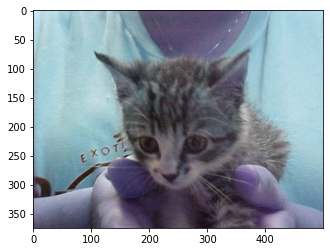
\includegraphics[width=0.48\textwidth]{Images/cat_1.png}
    \caption{Sample image from dataset.}
    \label{fig:sample-dataset}
\end{figure}

Image classification is where a computer can analyse an image and identify the ‘class’ the image falls under. (Or a probability of the image being part of a ‘class’.) A class is essentially a label, for instance, ‘car’, ‘animal’, ‘building’ and so on. 

This project aims to create multiple machine learning mdoels to predict if a photo given to the model is either a cat, or a dog. Three different network models were used to find the most efficient and accurate model for image classification.


\section{Dataset}
% Delete the text and write your Theory/ Background Information here:
%------------------------------------

For our goal, we are going to use the Cats and Dogs dataset that is given for the project. This dataset has a total of 25000 images, 12500 of them are cats, and the other 12500 are dogs. \par

These images are all informal pet images like the ones we usually have on our phones, and this is important because it means that our model will be more versatile. Otherwise, it would only be able to understand a pet type if the picture had a certain characteristic or was taken in a specific manner. \par

A sample image from the dataset can be seen at Figure 1.
\section{Models Used}
% Delete the text and write your Method(s) here:
%------------------------------------
\begin{figure}
    \centering
    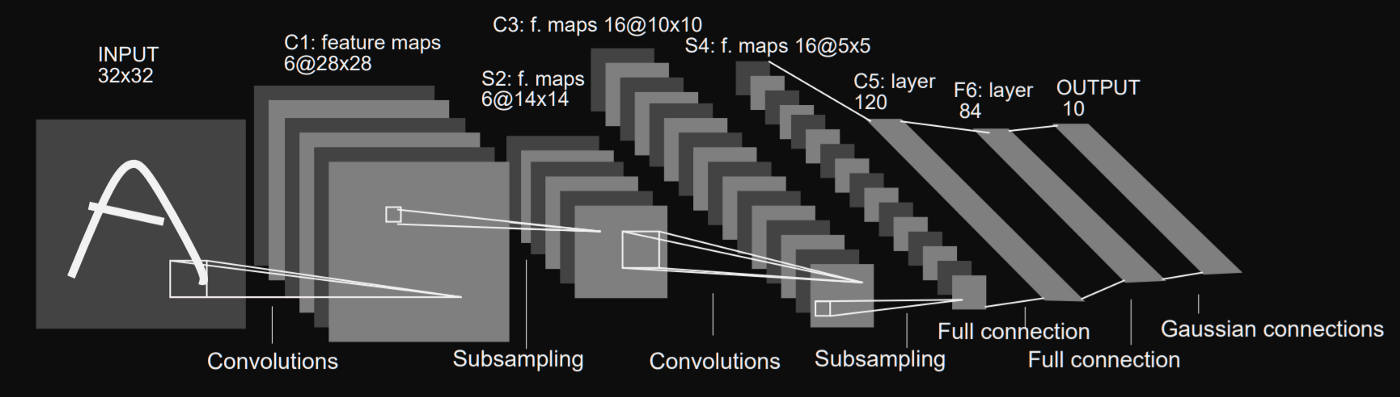
\includegraphics[width=0.48\textwidth]{Images/lenet_arcj.png}
    \caption{LeNet-5 Architecture}
    \label{fig:lenet-arch}
\end{figure}
\begin{figure}
    \centering
    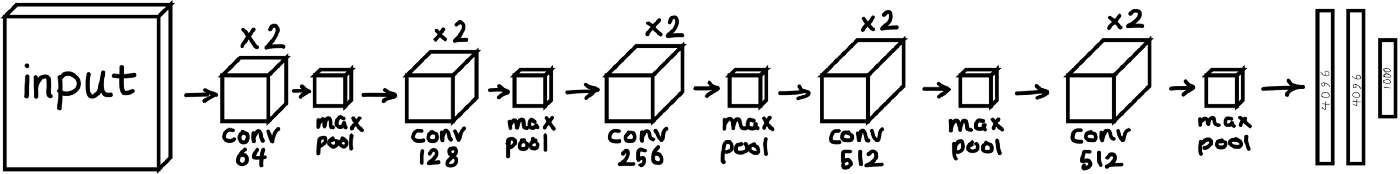
\includegraphics[width=0.48\textwidth]{Images/vgg-13-diag.png}
    \caption{Flow Diagram for VGG-13 Architecture}
    \label{fig:vgg-13-diag}
\end{figure}
\begin{figure}
    \centering
    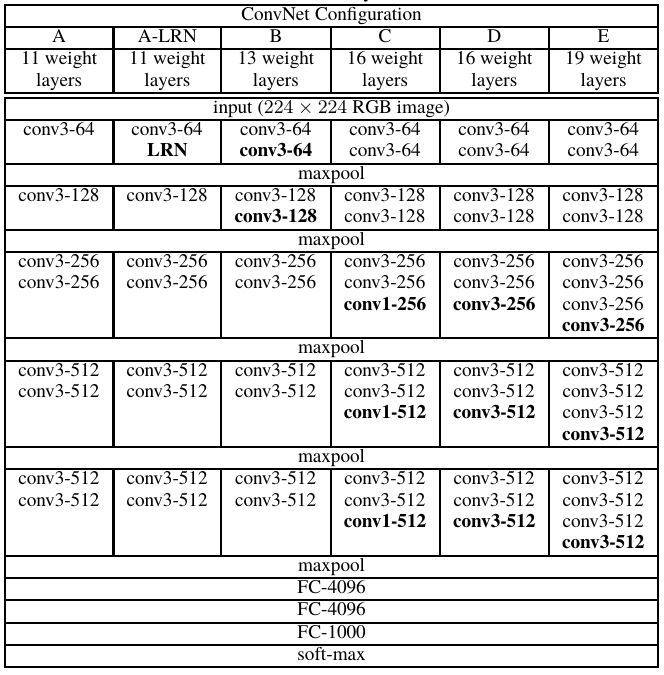
\includegraphics[width=0.48\textwidth]{Images/vgg_list.png}
    \caption{List Of VGG Architectures.}
    \label{fig:vgg-list}
\end{figure}
\subsection{VGG}
VGG stands for Visual Geometry Group; it is a standard deep Convolutional Neural Network (CNN) architecture with multiple layers. The “deep” refers to the number of layers with VGG-16 or VGG-19 consisting of 16 and 19 convolutional layers.\par

The VGG architecture is the basis of ground-breaking object recognition models. Developed as a deep neural network, the VGGNet also surpasses baselines on many tasks and datasets beyond ImageNet. Moreover, it is now still one of the most popular image recognition architectures.\par

This study uses VGG-3 and VGG-13 as the two different machine learning networks.\par 
To make the study simple, VGG-13 was chosen as it is the easier to implement out of multi layered machine learning networks. Following the same logic VGG-16 and VGG-19 can also be easily implemented for the dataset. \cref{fig:vgg-list} describes VGG-13 and others in a table. \par
VGG13 is model B in  \cref{fig:vgg-list}. A diagram can be found in \cref{fig:vgg-13-diag} to simplify how VGG-13 works in back.
\subsection{LeNet}

LeNet was introduced in the research paper “Gradient-Based Learning Applied To Document Recognition” in the year 1998 by Yann LeCun, Leon Bottou, Yoshua Bengio, and Patrick Haffner. Many of the listed authors of the paper have gone on to provide several significant academic contributions to the field of deep learning.\par
LeNet-5 CNN architecture is made up of 7 layers. The layer composition consists of 3 convolutional layers, 2 subsampling layers and 2 fully connected layers. \par

\cref{fig:lenet-arch} shows a depiction of the LeNet-5 architecture, as illustrated in the original paper. \par

The LeNet architecture is an excellent “first architecture” for Convolutional Neural Networks. LeNet is small and easy to understand — yet large enough to provide interesting results. Furthermore, the combination of LeNet + MNIST is able to run on the CPU, making it easy for beginners to take their first step in Deep Learning and Convolutional Neural Networks. \par

\subsection{CNN}
A convolutional neural network (CNN) is a type of artificial neural network used in image recognition and processing that is specifically designed to process pixel data.\par

CNNs are powerful image processing, artificial intelligence (AI) that use deep learning to perform both generative and descriptive tasks, often using machine vison that includes image and video recognition, along with recommender systems and natural language processing (NLP).\par

A neural network is a system of hardware and/or software patterned after the operation of neurons in the human brain. Traditional neural networks are not ideal for image processing and must be fed images in reduced-resolution pieces. CNN have their “neurons” arranged more like those of the frontal lobe, the area responsible for processing visual stimuli in humans and other animals. The layers of neurons are arranged in such a way as to cover the entire visual field avoiding the piecemeal image processing problem of traditional neural networks.\par

 \subsection{k-Fold Cross Validation}
 Cross-validation is a resampling procedure used to evaluate machine learning models on a limited data sample. \par

The procedure has a single parameter called k that refers to the number of groups that a given data sample is to be split into. As such, the procedure is often called k-fold cross-validation. When a specific value for k is chosen, it may be used in place of k in the reference to the model, such as k=10 becoming 10-fold cross-validation.\par

Cross-validation is primarily used in applied machine learning to estimate the skill of a machine learning model on unseen data. That is, to use a limited sample in order to estimate how the model is expected to perform in general when used to make predictions on data not used during the training of the model.\par
\begin{figure}
    \centering
    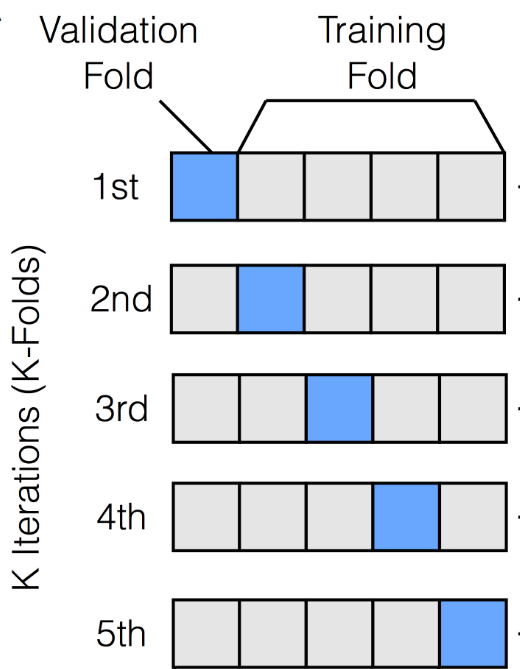
\includegraphics[width=0.48\textwidth]{Images/cross_validation.png}
    \caption{5-Fold Cross Validation Visualization}
    \label{fig:cross_validation}
\end{figure}
For cross validation kfold method from sklearn library is used. KFold method automatizises the cross validation that we do in our models' training. Figure  \cref{fig:cross_validation} represents how our 5 fold cross validation works in action. \par
How the K-Fold Cross validation is implemented is discussed in Appendix section of this paper.\par

\section{Parameters}
In the study, different parameters are used in each machine learning network. These are in order:
\subsection{Batch Size}
The batch size is a hyperparameter that defines the number of samples to work through before updating the internal model parameters.\par

Think of a batch as a for-loop iterating over one or more samples and making predictions. At the end of the batch, the predictions are compared to the expected output variables and an error is calculated. From this error, the update algorithm is used to improve the model, e.g. move down along the error gradient.\par
\subsection{SGD}
Stochastic Gradient Descent, or SGD for short, is an optimization algorithm used to train machine learning algorithms, most notably artificial neural networks used in deep learning. \par
The job of the algorithm is to find a set of internal model parameters that perform well against some performance measure such as logarithmic loss or mean squared error. \par
Optimization is a type of searching process and you can think of this search as learning. The optimization algorithm is called “gradient descent“, where “gradient” refers to the calculation of an error gradient or slope of error and “descent” refers to the moving down along that slope towards some minimum level of error. \par
\subsection{Epoch}
The number of epochs is a hyperparameter that defines the number times that the learning algorithm will work through the entire training dataset. \par

One epoch means that each sample in the training dataset has had an opportunity to update the internal model parameters. An epoch is comprised of one or more batches. For example, as above, an epoch that has one batch is called the batch gradient descent learning algorithm.\par
\section{Data Processing}
% Delete the text and write your Results here:
%------------------------------------
The dataset of cats and dogs are compromised of 25000 images that are 400 by 500 photos. \par
The first step of generating the training data is grayscaling it. Grayscaling is done by OpenCV's IMREAD\_GRAYSCALE option. \par
\begin{figure}
    \centering
    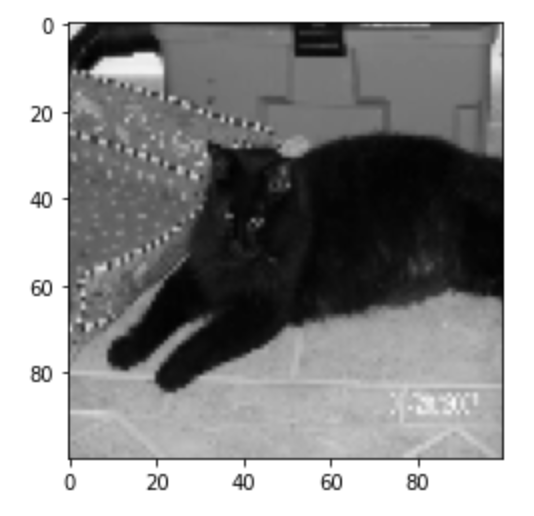
\includegraphics[width=0.48\textwidth]{Images/cat_subres.png}
    \caption{A gray and white, subsampled photo of a cat}
    \label{fig:cat_subres}
\end{figure}
After grayscaling the images, the next step is resizing it. For resizing, a 128 by 128 resolution were chosen, because it was the better resolution for quality and size. The resizing task was also done by OpenCV. \par
Processed dataset is split by 90\% train and 10\% test for checking the accuracies of each network and their one zero losses. \par
After these steps, the images are saved to use in our training and foldings. 
\section{Results}
% Delete the text and write your Discussion here:
%------------------------------------

Here are the results that's collected for each of our machine learning networks 
\begin{figure}
    \centering
    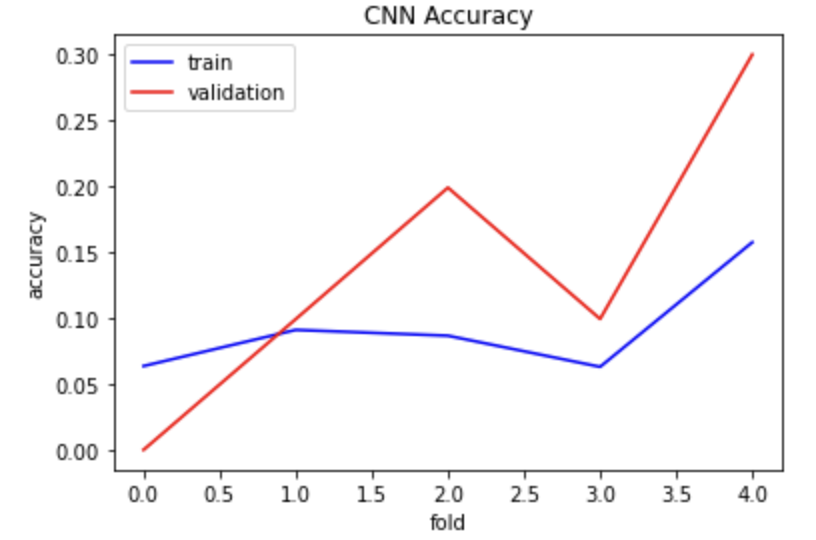
\includegraphics[width=0.48\textwidth]{Images/cnn.png}
    \caption{Validation Accuracies of CNN}
    \label{fig:NTNU-letters}
\end{figure}
\subsection{CNN}
Our CNN model performed the best out of the networks that we used. After 5 folds, the validation accuracies were around 70\% and our one zero losses are 0.15 mark. For the training of CNN, RMSprop were used for the optimiser.For the learning rate of RMSProp, 0.001 was chosen because with lower learning rates yielded lower validation accuracies. And for our each fold, 10 epoches with 50 steps were done.\par

Epoch is left at 10, because the more epoches were executed, the overfitting started to occur on the model. Used CNN network has 3 layers with pooling inbetween. For each convolusional layer, relu activation was used differentiate between the inputs and outputs.
\begin{figure}
    \centering
    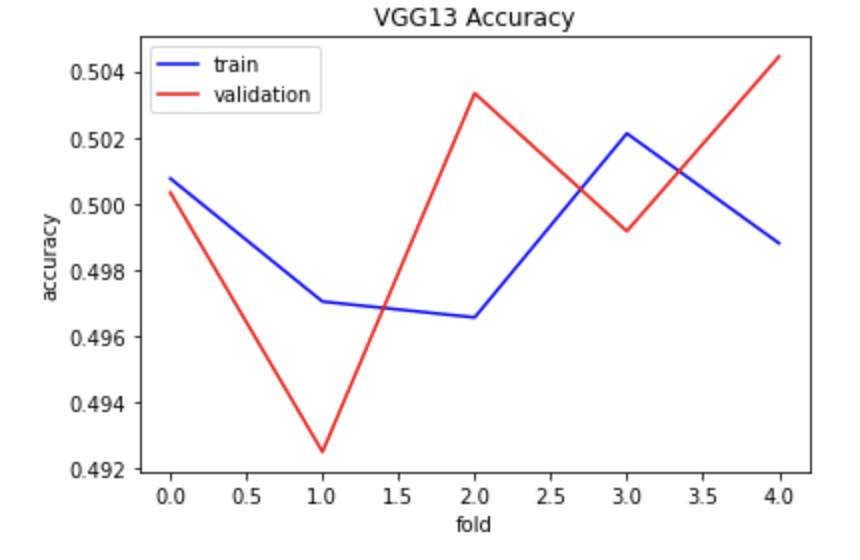
\includegraphics[width=0.48\textwidth]{Images/vgg13.png}
    \caption{Validation Accuracies of VGG13}
    \label{fig:NTNU-letters}
\end{figure}
\subsection{VGG13}
Our VGG13 is the second best performant model out of our models. It performed worse than the CNN model, because the VGG13 networks is not the best suited for black and white images. After 5 folds, the validation accuracies were around 60\% and our one zero losses are 0.35 mark. For the training of VGG13, RMSProp with a lower learning rate were used for the optimiser. And for our each fold, 10 epoches with no steps were done.


\begin{figure}
    \centering
    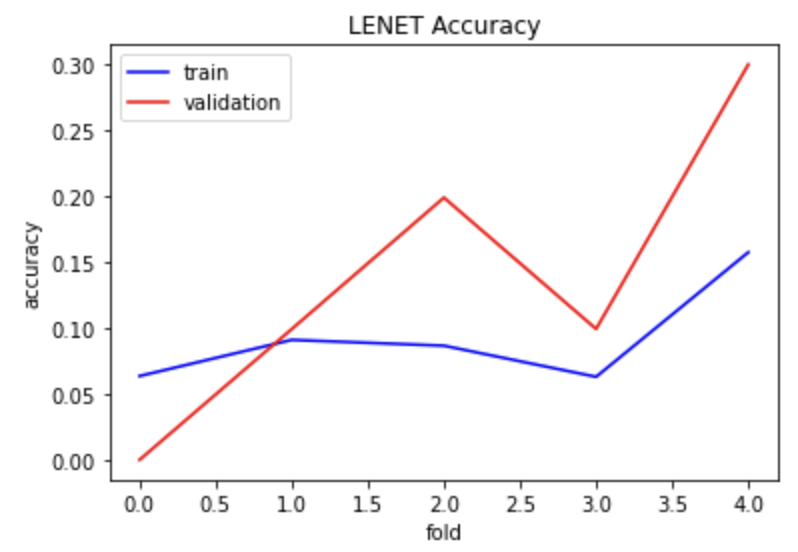
\includegraphics[width=0.48\textwidth]{Images/lenet.png}
    \caption{Validation Accuracies of LeNet}
    \label{fig:NTNU-letters}
\end{figure}
\subsection{LeNet}
Our LeNet is the third best performant model out of our models. It performed rather poorly because of the fact that LeNet needs images to be high quality as much as possible. After 5 folds, the validation accuracies were around 30\% and our one zero losses are 0.70 mark. For the training of LeNet, adam with a lower learning rate were used for the optimiser. 20 epoches were done with no incremental steps were done.
\begin{figure}
    \centering
    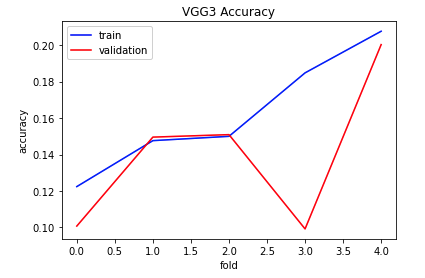
\includegraphics[width=0.48\textwidth]{Images/vgg3.png}
    \caption{Validation Accuracies of VGG3}
    \label{fig:NTNU-letters}
\end{figure}
\subsection{VGG3}
VGG3 is the last network implementation that we used. VGG3 was not suited for our testings, and the results that we collected shows it. We got at max 20\% validation accuracy rate, and the one zero loss is nearly 1. VGG3 is not a good choice for informal photos such as what we have in our dataset, because of the fact that the layers are too small to handle informal photos that are big in resolution. \par

After finishing all the tests, we can conclude that CNN architecture with 8 starting layers with the RMSProp optimiser was the best choice for the kind of dataset that we used. The results may have varied if the images were not black and white, or if the images were higher resolution from what we chose.


%\clearpage                                     % Sometimes you want the rest on separate pages.
%\section*{Acknowledgements}
% Delete the text and write Acknowledgements here (not required, can be omitted):
% Comment out ' \section*{Acknowledgements}
% Delete the text and write Acknowledgements here (not required, can be omitted):
% Comment out ' \section*{Acknowledgements}
% Delete the text and write Acknowledgements here (not required, can be omitted):
% Comment out ' \input{Text/Acknowledgements} ' to remove this section.
%------------------------------------


Acknowledgements (nb. takksigelser, nn. takkseiingar) is not a requirement in a laboratory report. However, it is used in most 
scientific articles. It looks more professional and adds some ``extra spice'' to your report. Here is an example: \par
The authors would like to thank Dr. Ola Normann at the
University of Oslo for assistance with the SIMS-analysis
and Dr. Kari Normann at NTNU for fruitful discussions
and support concerning melt spinning of silicon. This work
was financially supported by the Norwegian research council and the Norwegian PhD Network on Nanotechnology
for Microsystems.
 ' to remove this section.
%------------------------------------


Acknowledgements (nb. takksigelser, nn. takkseiingar) is not a requirement in a laboratory report. However, it is used in most 
scientific articles. It looks more professional and adds some ``extra spice'' to your report. Here is an example: \par
The authors would like to thank Dr. Ola Normann at the
University of Oslo for assistance with the SIMS-analysis
and Dr. Kari Normann at NTNU for fruitful discussions
and support concerning melt spinning of silicon. This work
was financially supported by the Norwegian research council and the Norwegian PhD Network on Nanotechnology
for Microsystems.
 ' to remove this section.
%------------------------------------


Acknowledgements (nb. takksigelser, nn. takkseiingar) is not a requirement in a laboratory report. However, it is used in most 
scientific articles. It looks more professional and adds some ``extra spice'' to your report. Here is an example: \par
The authors would like to thank Dr. Ola Normann at the
University of Oslo for assistance with the SIMS-analysis
and Dr. Kari Normann at NTNU for fruitful discussions
and support concerning melt spinning of silicon. This work
was financially supported by the Norwegian research council and the Norwegian PhD Network on Nanotechnology
for Microsystems.
                   % Comment out to exclude the Acknowledgements section

%%%%%%%%%%%%%%%%%%%%%%%%%%%%%%%%%%%%%%%%

% Bibliography
%--------------------
\printbibliography

%\clearpage                                     % Sometimes it is useful to have appendix on separate page.
%\onecolumn                                     % If you want 1 column for appendix.
\appendix
% Delete the text and write Appendix here (not required, can be omitted):
% Comment out ' \appendix
% Delete the text and write Appendix here (not required, can be omitted):
% Comment out ' \appendix
% Delete the text and write Appendix here (not required, can be omitted):
% Comment out ' \input{Text/Appendix} ' to remove this section.
%------------------------------------


\section{Additional Information}
\subsection{Python codes}
All of the data processing and network trainings are done on Cats\_And\_Dogs.ipynb file. In \cref{listing:1} a basic implementation of cross validation can be seen. 
% because I have loaded varioref and cleveref (in that order) varioref has "become clever", and you can
% use \Vref{} in the start of a sentence.



\begin{listing}[!htb]

\inputminted[%
firstline=1, 
lastline=15,
bgcolor=LightGray,
breaklines,
breaksymbolleft={},
breakindent={15pt}
]{python}{Code/Python/kfold.py}

\caption{Basic K-Fold implementation}
\label{listing:1}
\end{listing}

The code from \cref{listing:1} was displayed using a \verb+.py+ file. Since the lines are not numbered in this code example, you can copy and paste the code from the PDF into python without many issues (does however need to correct indents). \par
The way cross folding that is implemented in the notebook is vastly different from what its written on here. This code is just an example for it.\par

\section{Model Summaries}
\begin{figure}
    \centering
    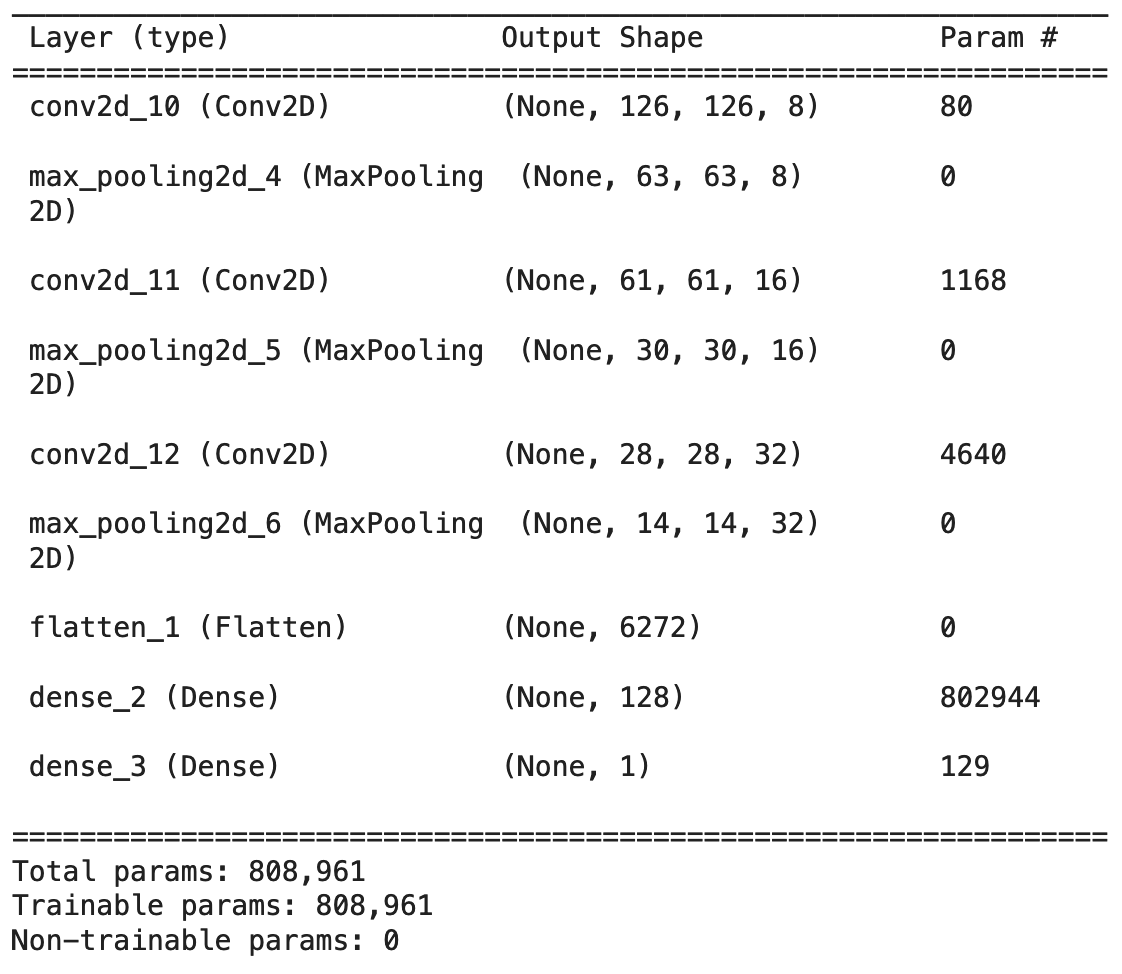
\includegraphics[width=0.48\textwidth]{Images/cnn_summary.png}
    \caption{CNN Summary}
    \label{fig:cnn_summary}
\end{figure}
\begin{figure}
    \centering
    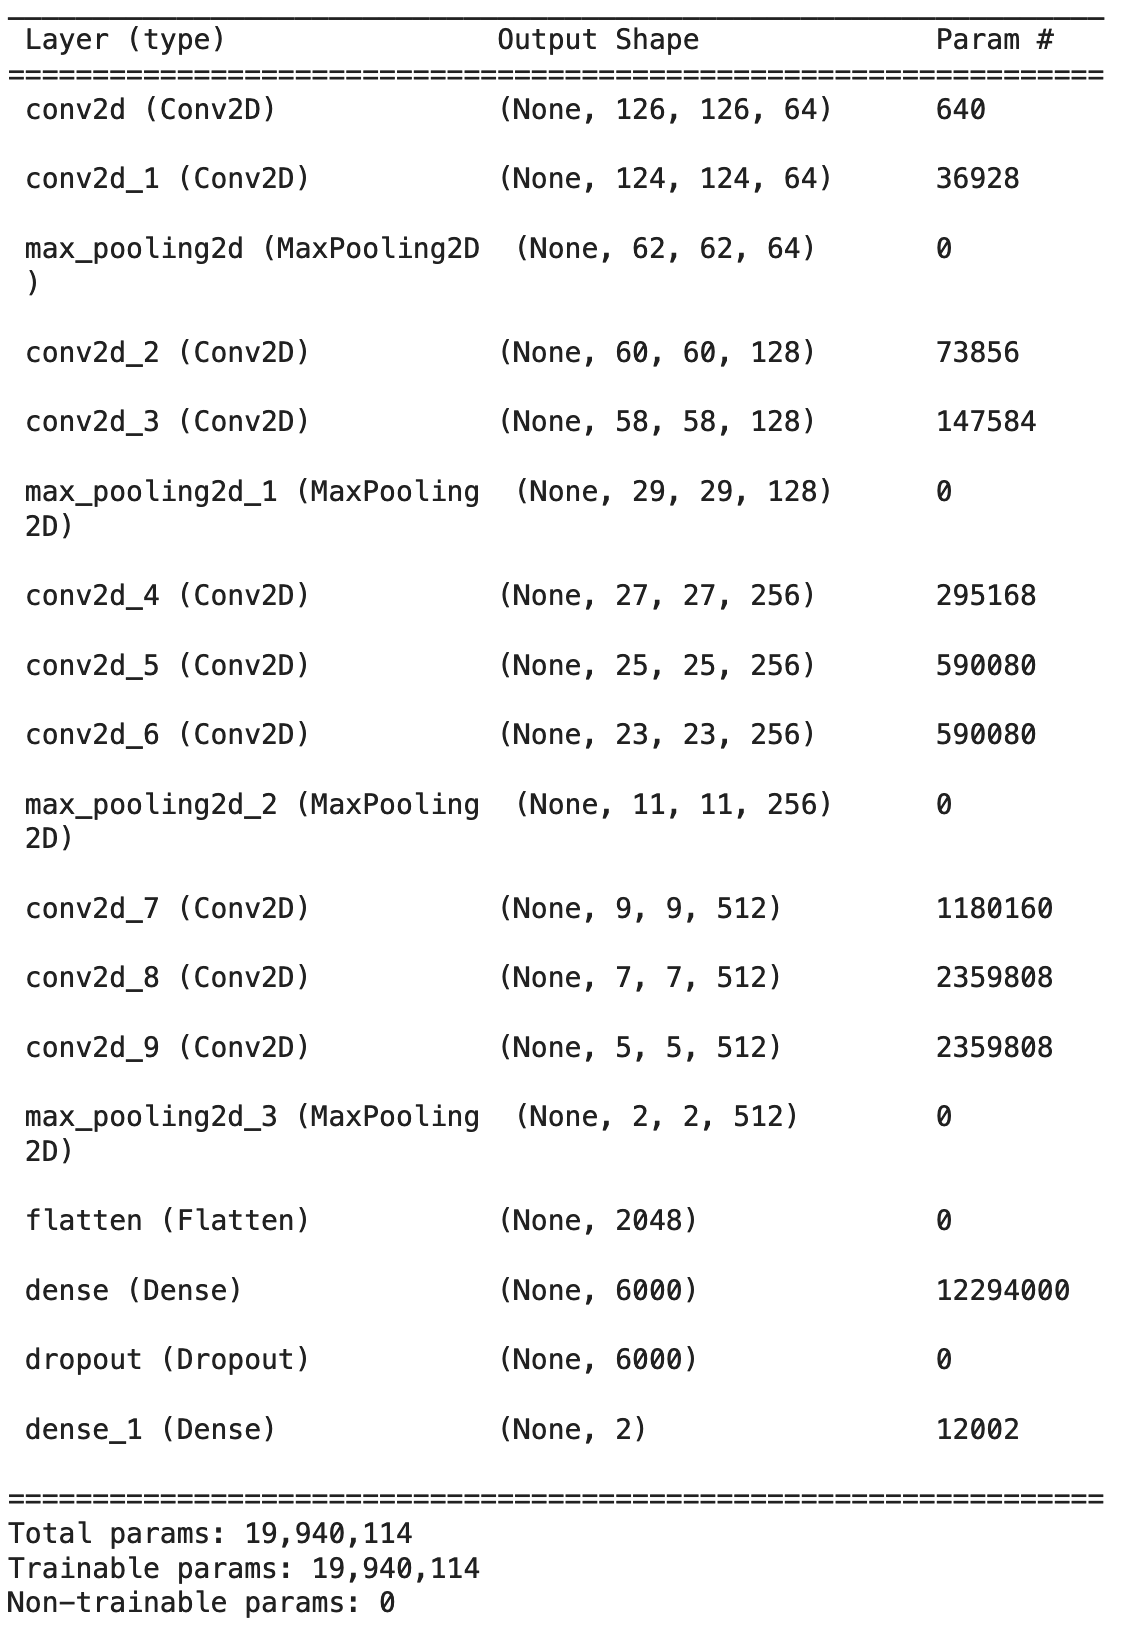
\includegraphics[width=0.48\textwidth]{Images/vgg13_summary.png}
    \caption{VGG13 Summary}
    \label{fig:vgg13_summary}
\end{figure}
\begin{figure}
    \centering
    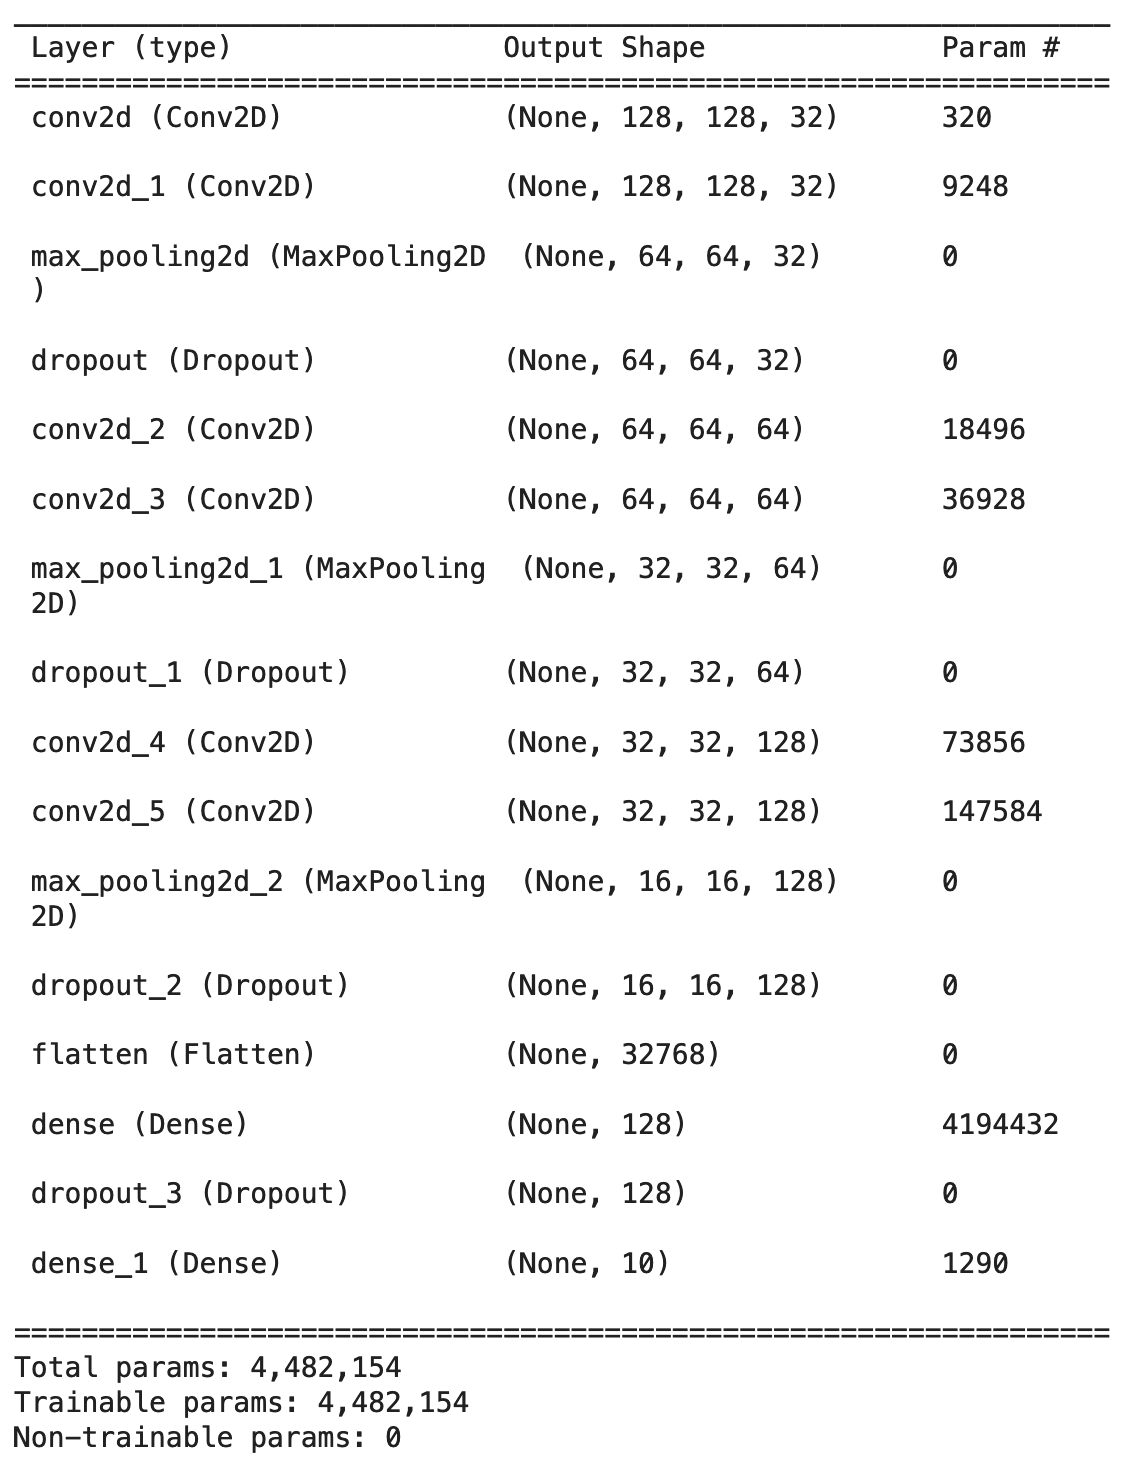
\includegraphics[width=0.48\textwidth]{Images/vgg3_summary.png}
    \caption{VGG3 Summary}
    \label{fig:vgg3_summary}
\end{figure}
\begin{figure}
    \centering
    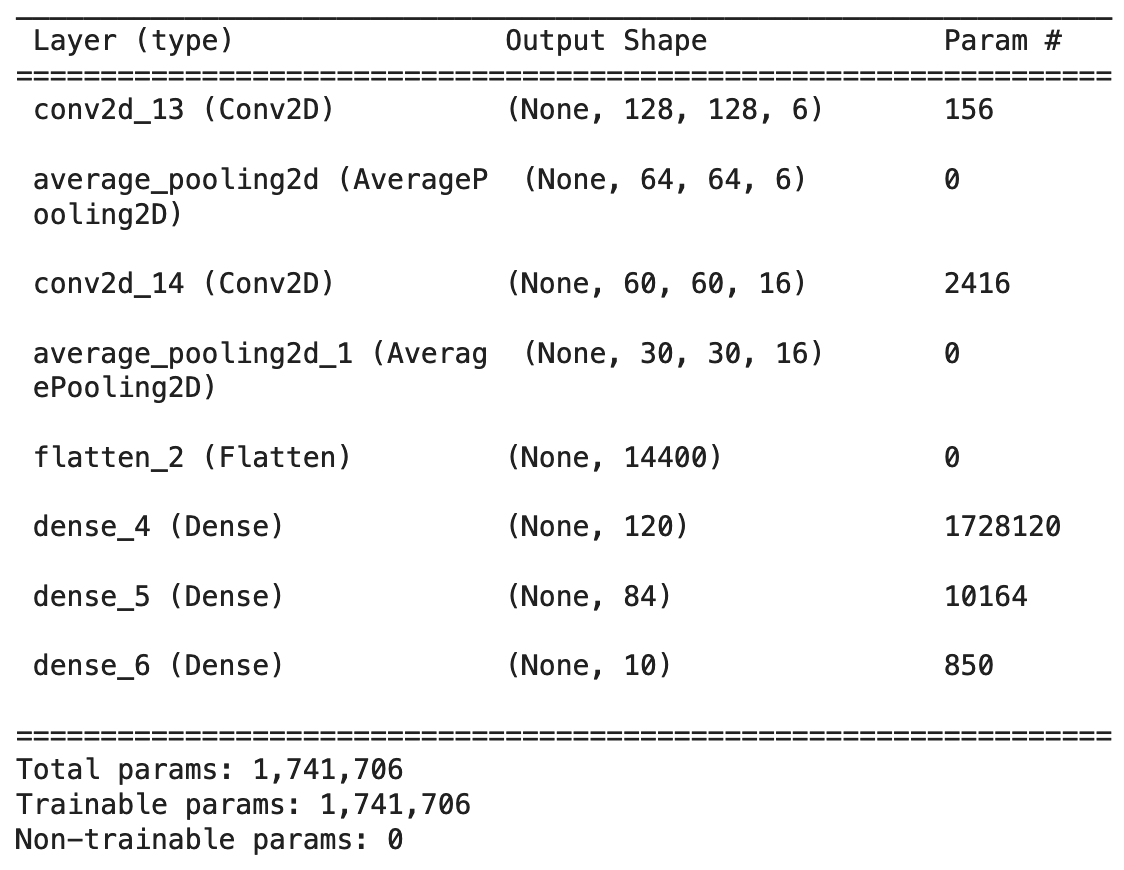
\includegraphics[width=0.48\textwidth]{Images/lenet_summary.png}
    \caption{LeNet Summary}
    \label{fig:lenet_summary}
\end{figure}
You can see the model summaries from figure \cref{fig:cnn_summary} to \cref{fig:lenet_summary}
 ' to remove this section.
%------------------------------------


\section{Additional Information}
\subsection{Python codes}
All of the data processing and network trainings are done on Cats\_And\_Dogs.ipynb file. In \cref{listing:1} a basic implementation of cross validation can be seen. 
% because I have loaded varioref and cleveref (in that order) varioref has "become clever", and you can
% use \Vref{} in the start of a sentence.



\begin{listing}[!htb]

\inputminted[%
firstline=1, 
lastline=15,
bgcolor=LightGray,
breaklines,
breaksymbolleft={},
breakindent={15pt}
]{python}{Code/Python/kfold.py}

\caption{Basic K-Fold implementation}
\label{listing:1}
\end{listing}

The code from \cref{listing:1} was displayed using a \verb+.py+ file. Since the lines are not numbered in this code example, you can copy and paste the code from the PDF into python without many issues (does however need to correct indents). \par
The way cross folding that is implemented in the notebook is vastly different from what its written on here. This code is just an example for it.\par

\section{Model Summaries}
\begin{figure}
    \centering
    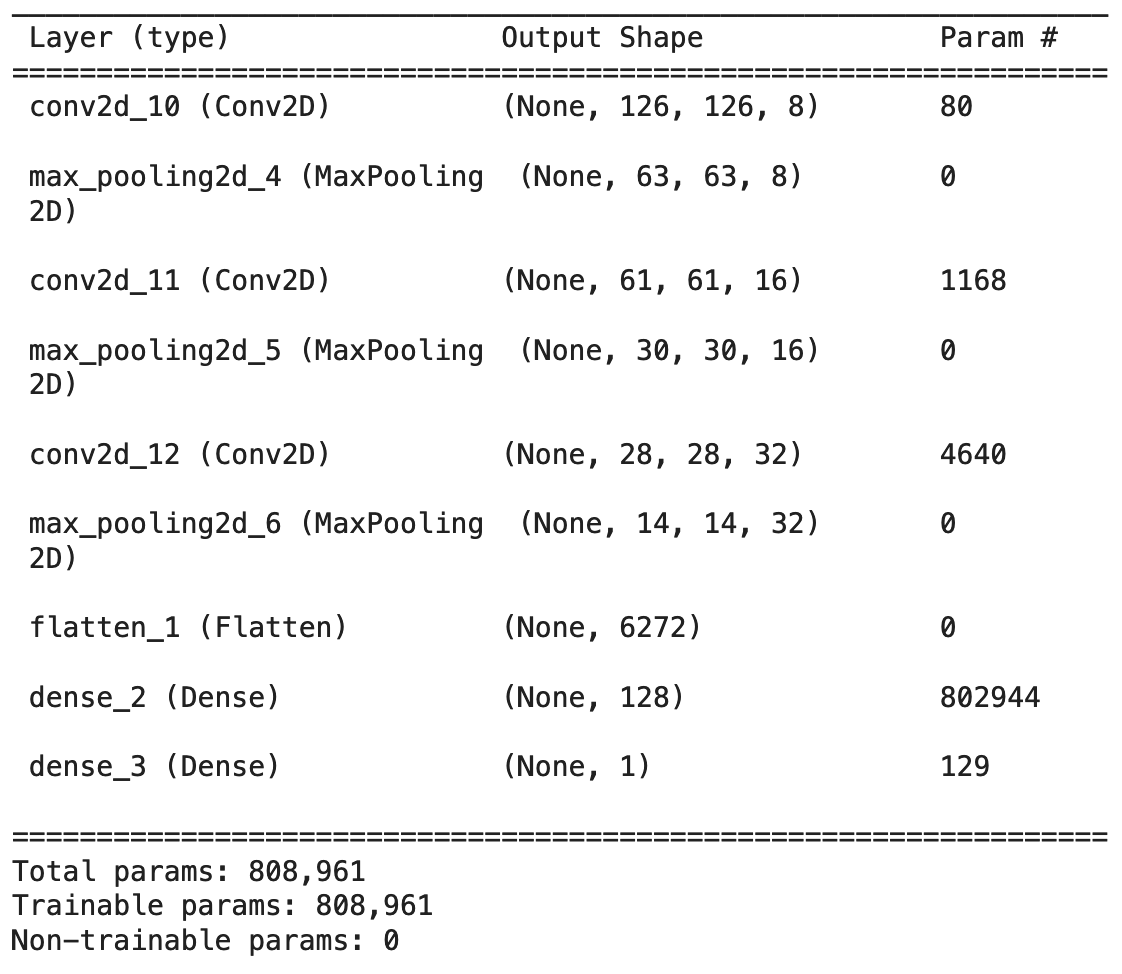
\includegraphics[width=0.48\textwidth]{Images/cnn_summary.png}
    \caption{CNN Summary}
    \label{fig:cnn_summary}
\end{figure}
\begin{figure}
    \centering
    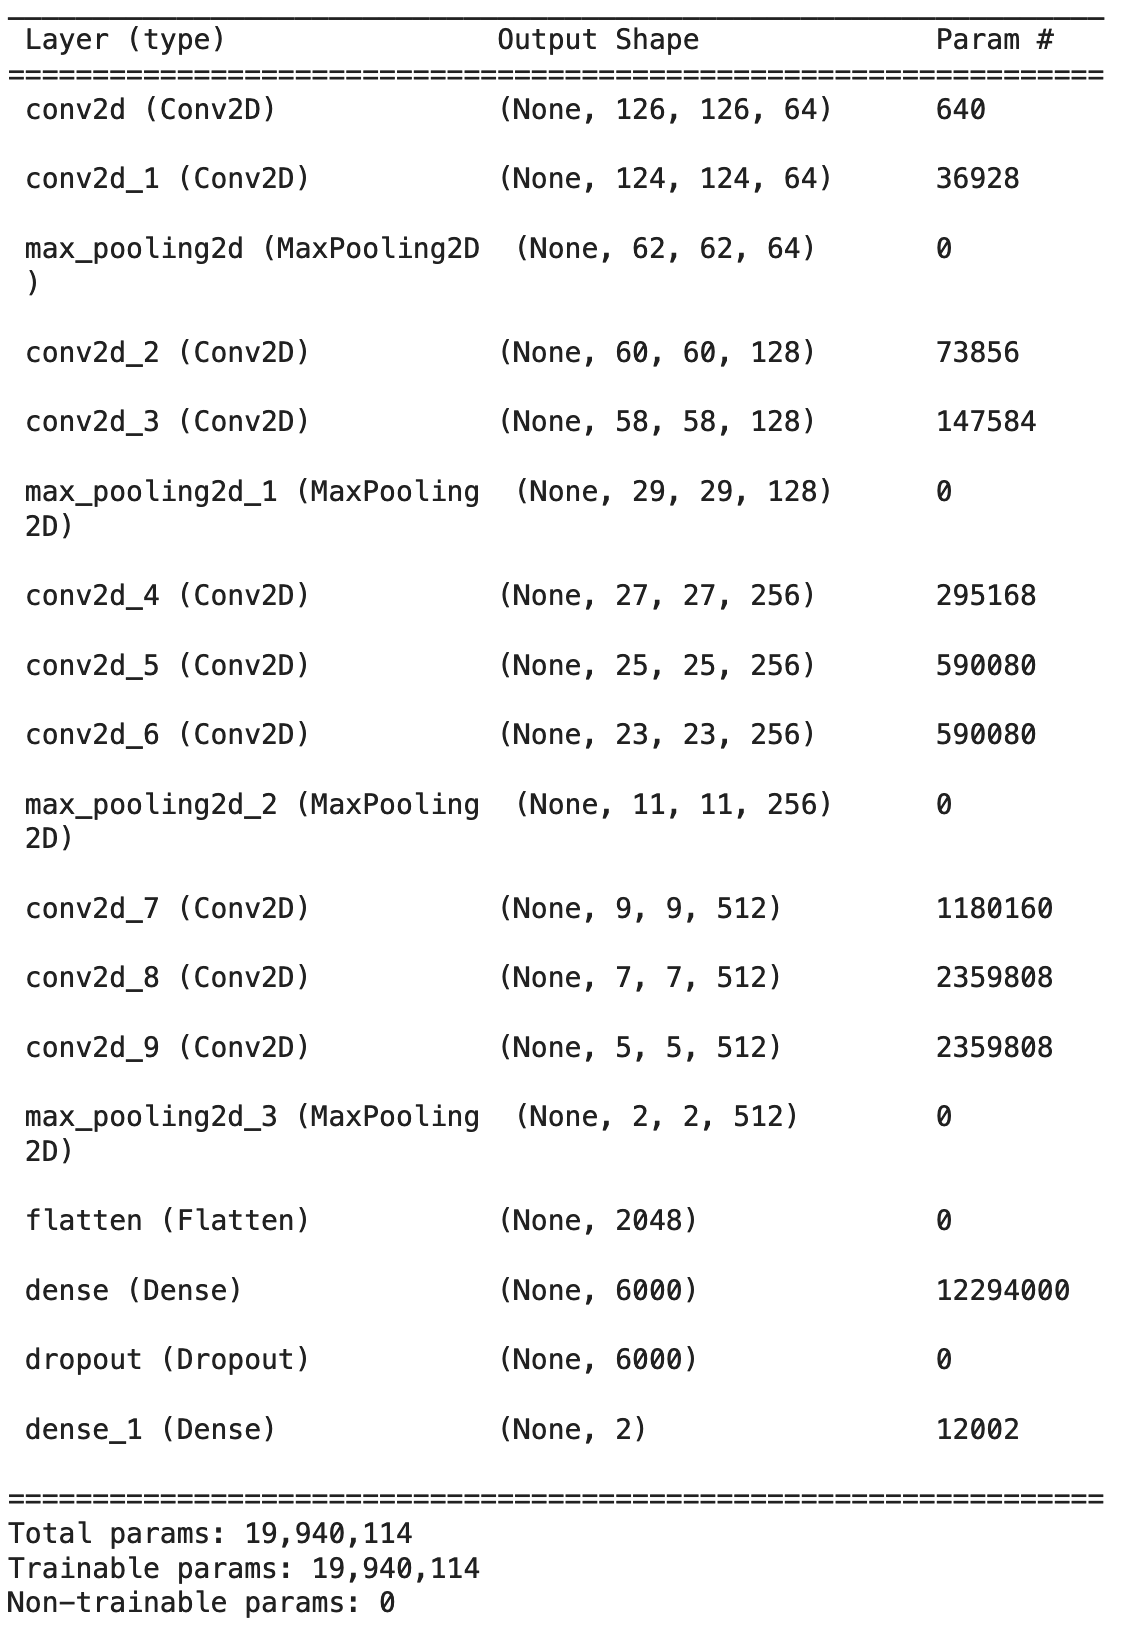
\includegraphics[width=0.48\textwidth]{Images/vgg13_summary.png}
    \caption{VGG13 Summary}
    \label{fig:vgg13_summary}
\end{figure}
\begin{figure}
    \centering
    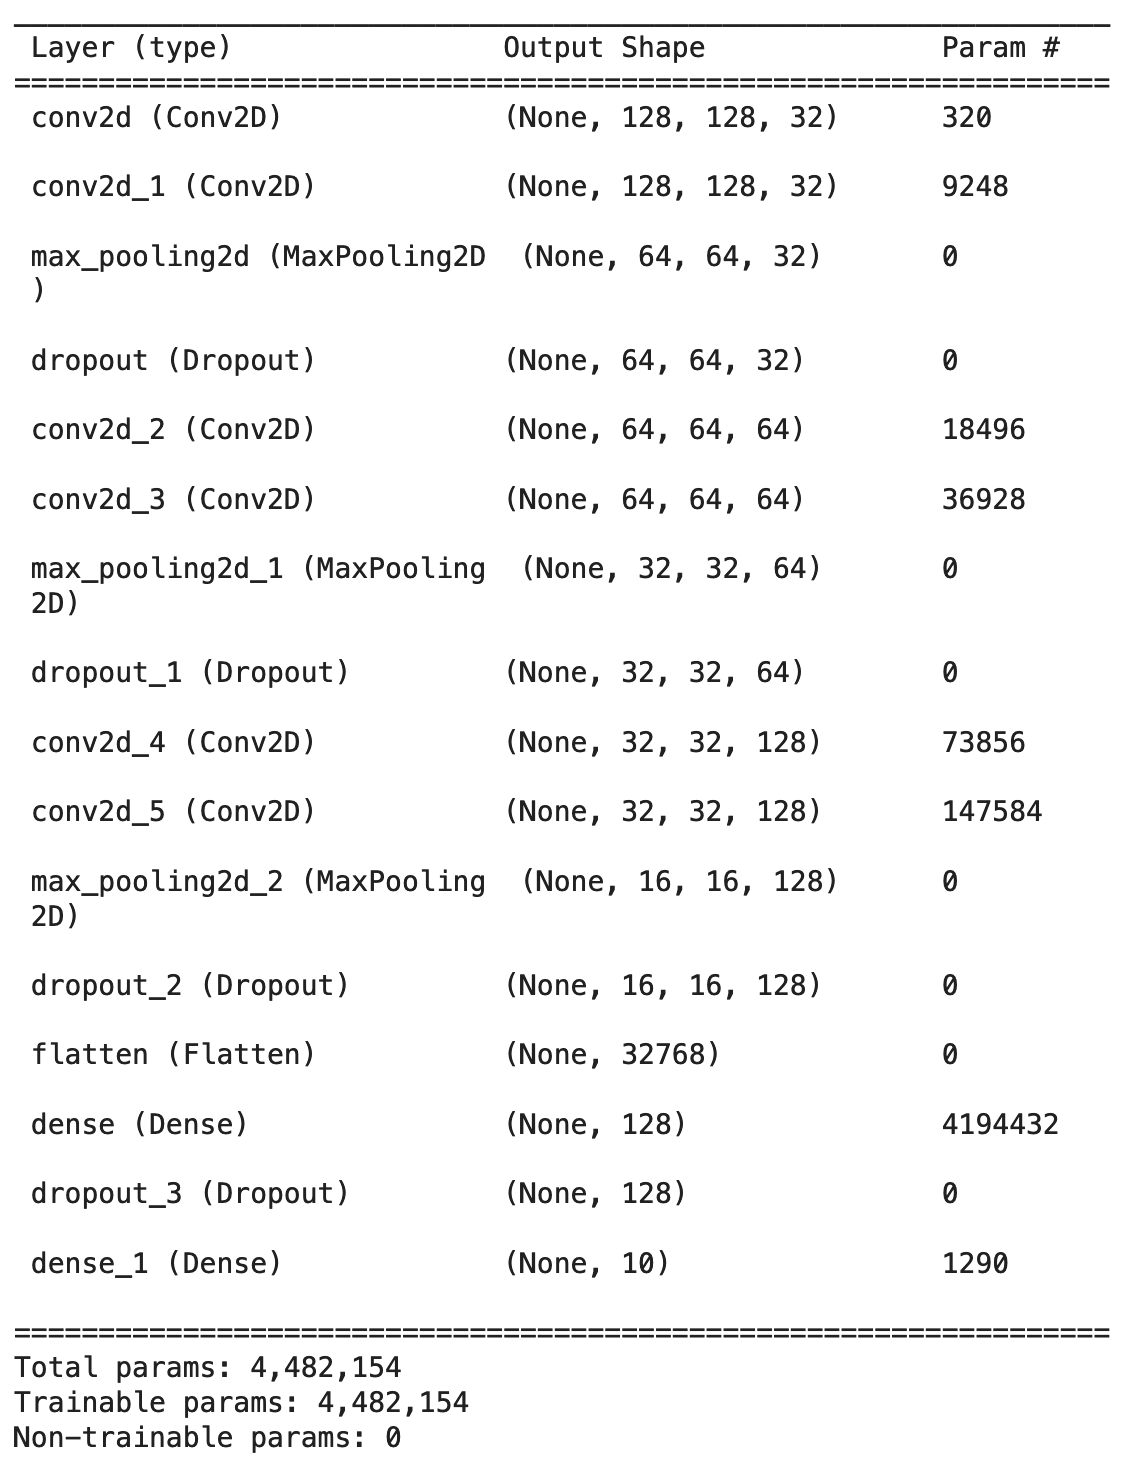
\includegraphics[width=0.48\textwidth]{Images/vgg3_summary.png}
    \caption{VGG3 Summary}
    \label{fig:vgg3_summary}
\end{figure}
\begin{figure}
    \centering
    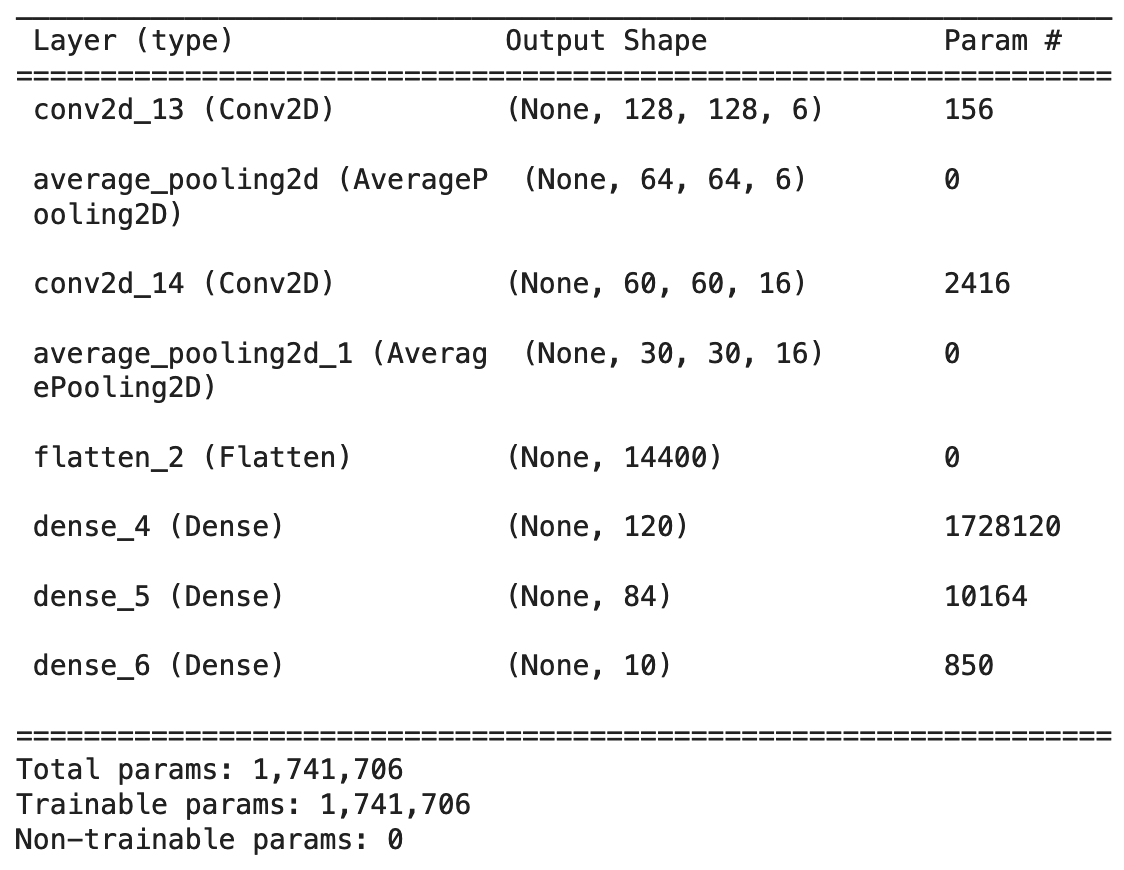
\includegraphics[width=0.48\textwidth]{Images/lenet_summary.png}
    \caption{LeNet Summary}
    \label{fig:lenet_summary}
\end{figure}
You can see the model summaries from figure \cref{fig:cnn_summary} to \cref{fig:lenet_summary}
 ' to remove this section.
%------------------------------------


\section{Additional Information}
\subsection{Python codes}
All of the data processing and network trainings are done on Cats\_And\_Dogs.ipynb file. In \cref{listing:1} a basic implementation of cross validation can be seen. 
% because I have loaded varioref and cleveref (in that order) varioref has "become clever", and you can
% use \Vref{} in the start of a sentence.



\begin{listing}[!htb]

\inputminted[%
firstline=1, 
lastline=15,
bgcolor=LightGray,
breaklines,
breaksymbolleft={},
breakindent={15pt}
]{python}{Code/Python/kfold.py}

\caption{Basic K-Fold implementation}
\label{listing:1}
\end{listing}

The code from \cref{listing:1} was displayed using a \verb+.py+ file. Since the lines are not numbered in this code example, you can copy and paste the code from the PDF into python without many issues (does however need to correct indents). \par
The way cross folding that is implemented in the notebook is vastly different from what its written on here. This code is just an example for it.\par

\section{Model Summaries}
\begin{figure}
    \centering
    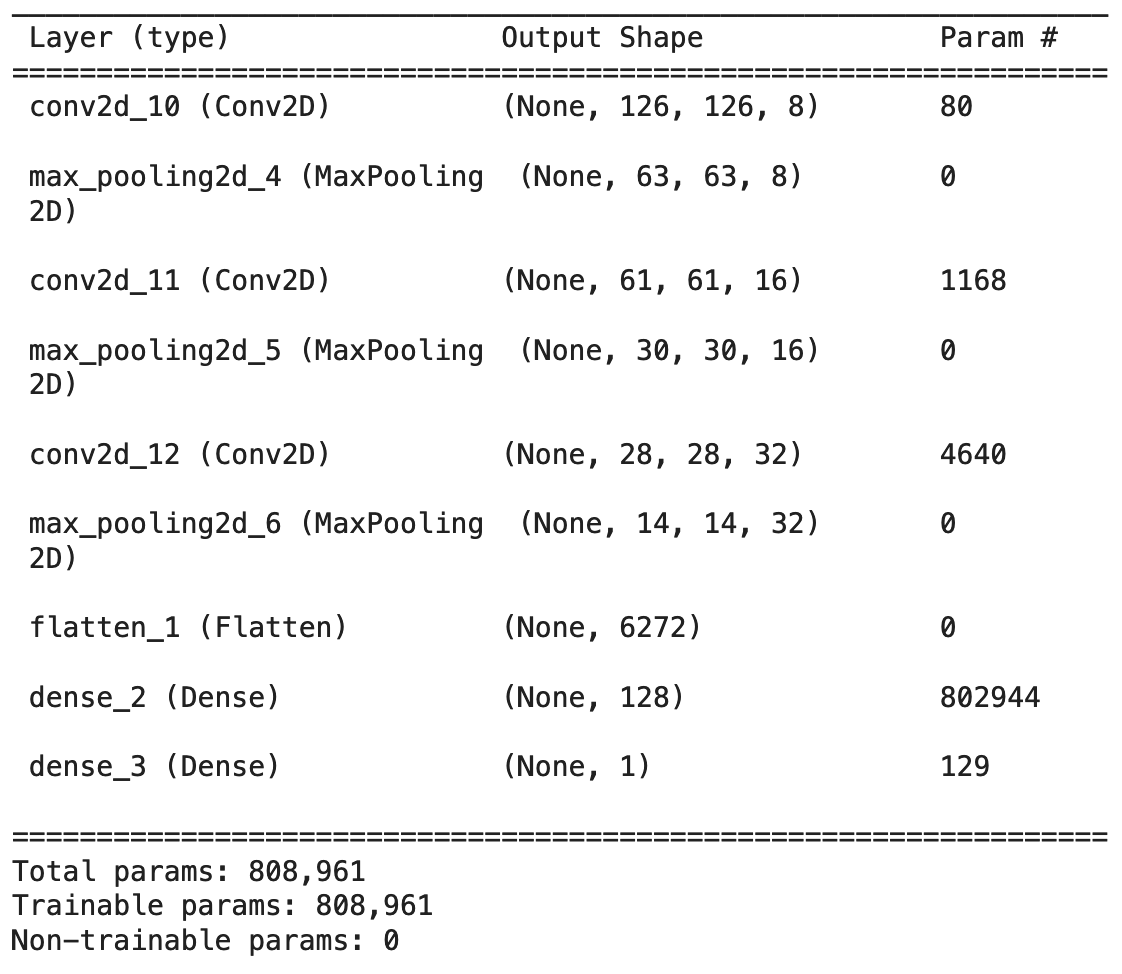
\includegraphics[width=0.48\textwidth]{Images/cnn_summary.png}
    \caption{CNN Summary}
    \label{fig:cnn_summary}
\end{figure}
\begin{figure}
    \centering
    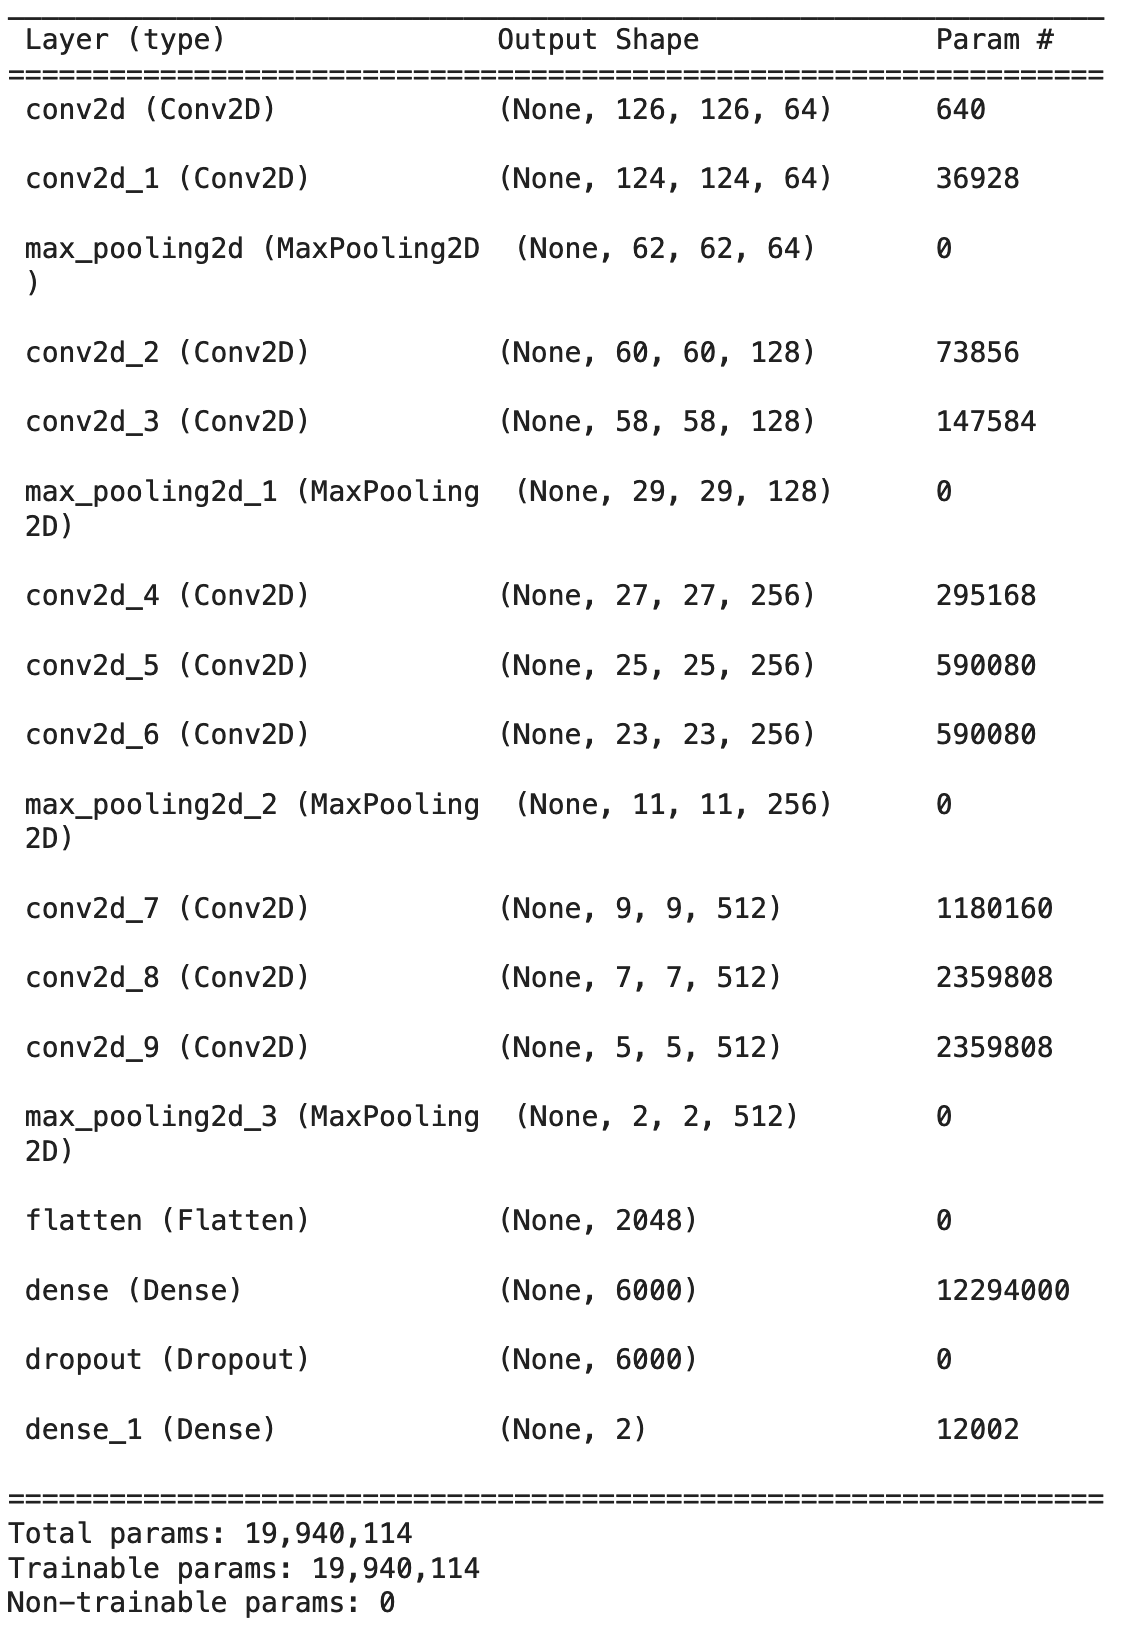
\includegraphics[width=0.48\textwidth]{Images/vgg13_summary.png}
    \caption{VGG13 Summary}
    \label{fig:vgg13_summary}
\end{figure}
\begin{figure}
    \centering
    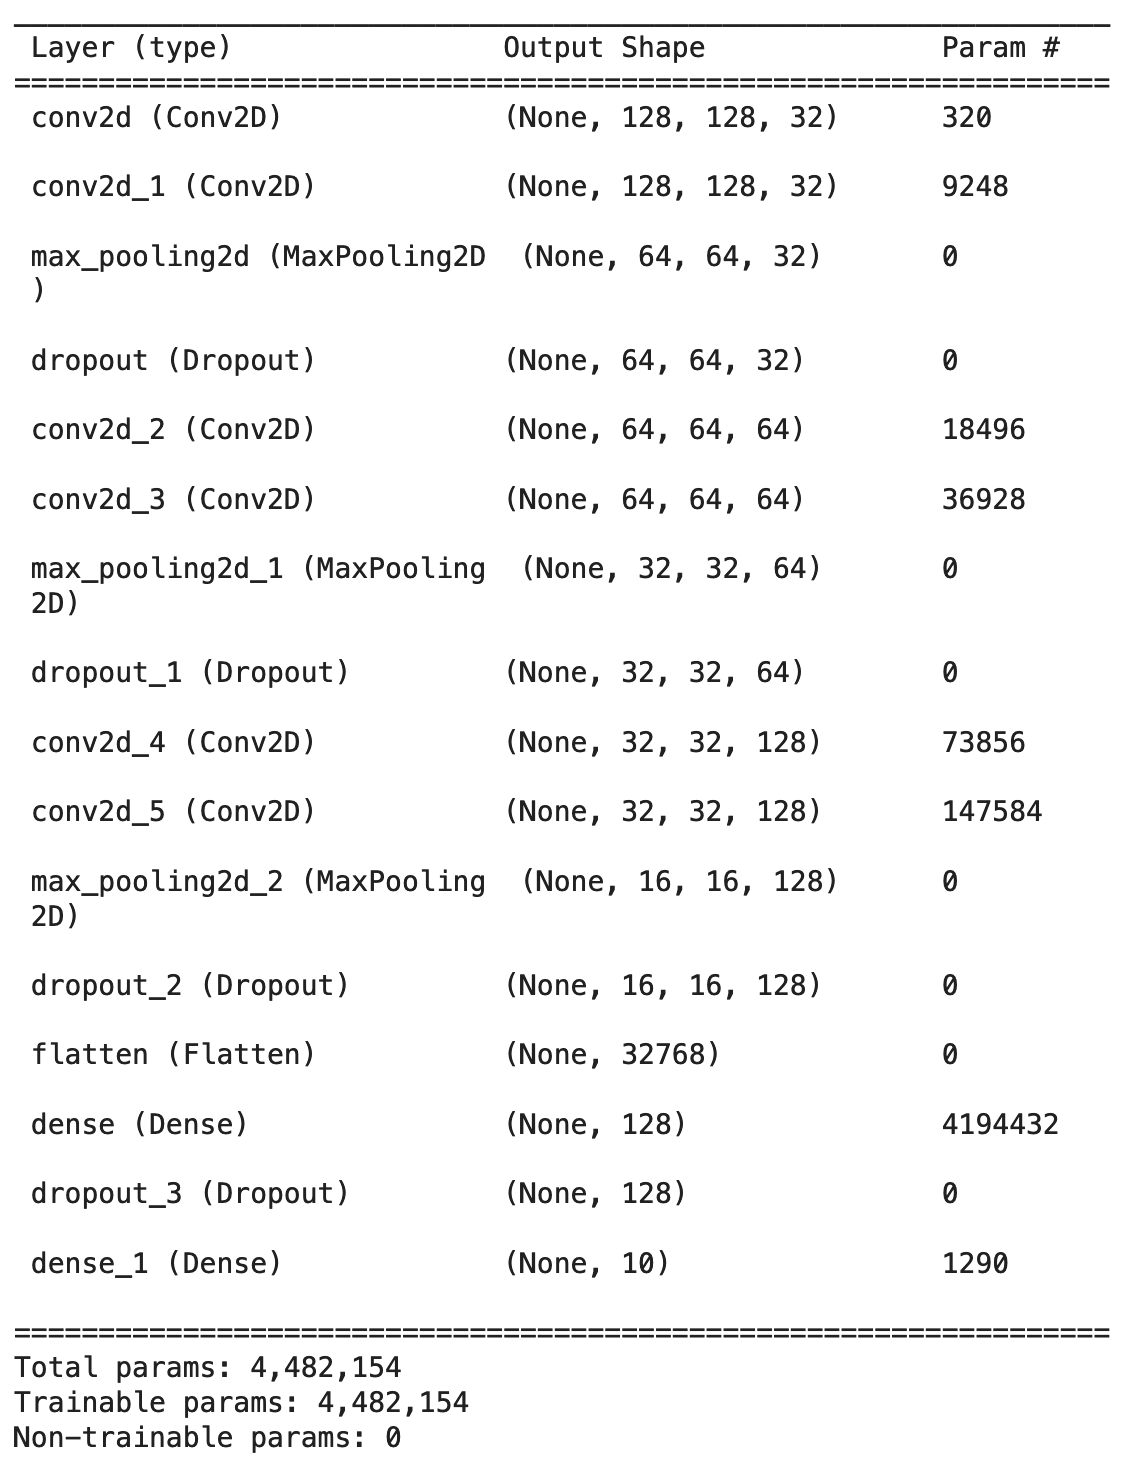
\includegraphics[width=0.48\textwidth]{Images/vgg3_summary.png}
    \caption{VGG3 Summary}
    \label{fig:vgg3_summary}
\end{figure}
\begin{figure}
    \centering
    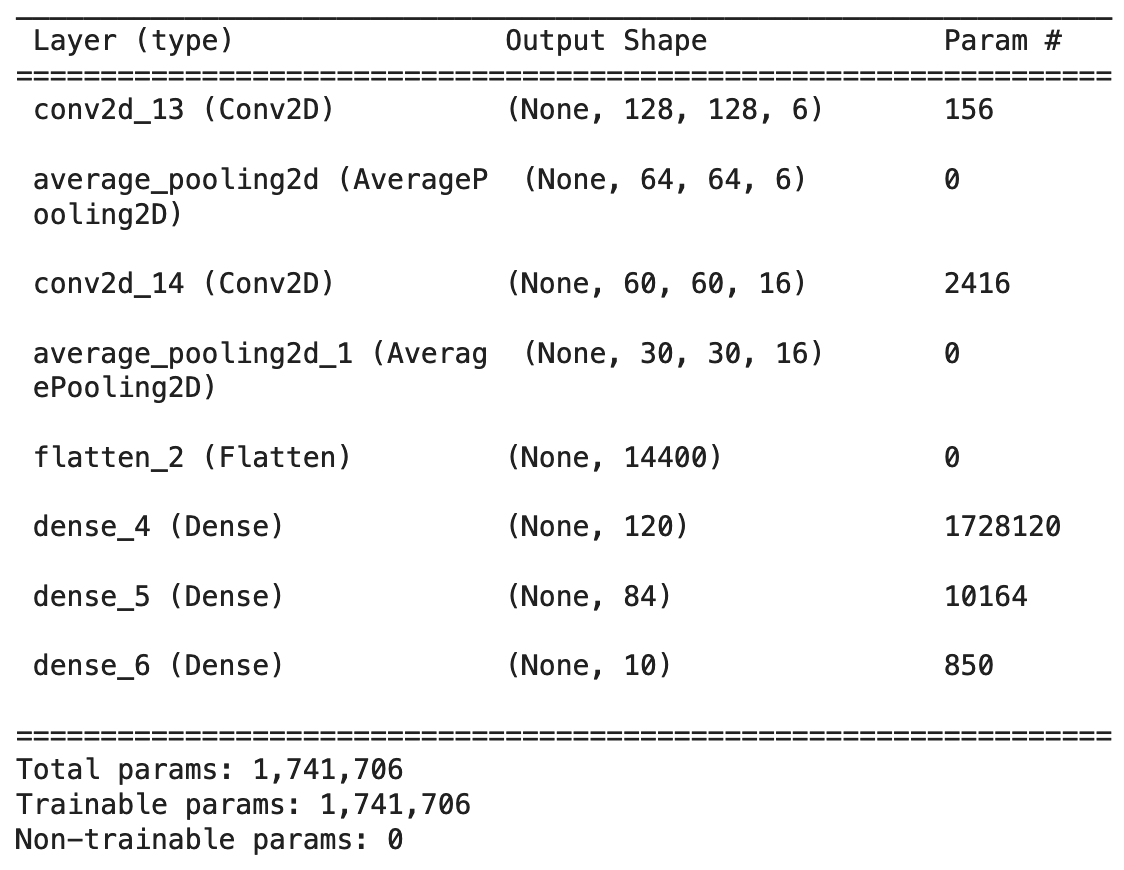
\includegraphics[width=0.48\textwidth]{Images/lenet_summary.png}
    \caption{LeNet Summary}
    \label{fig:lenet_summary}
\end{figure}
You can see the model summaries from figure \cref{fig:cnn_summary} to \cref{fig:lenet_summary}
                           % Comment out to exclude appendix

\end{document}

% Copyright Remarks:
%--------------------

% Copyright holder: Vebjørn S. Førde, copyright: CC BY 4.0
% Note: The author of this template is also the copyright holder.

% Below is an explanation of the CC BY 4.0. Additional statements/ 
% clarifications made by the author/copyright holder are marked with *.

% YOU ARE FREE TO:
% Share — copy and redistribute the material in any medium or format
% Adapt — remix, transform, and build upon the material
% for any purpose, even commercially.

% UNDER THE FOLLOWING TERMS:
% Attribution* — You must give appropriate credit, provide a link to the license,
% and indicate if changes were made. You may do so in any reasonable manner, but 
% not in any way that suggests the licensor endorses you or your use.

% *Note: I do not need credit when the template is used to make a PDF document
% that is then distributed (like handing in a lab report). However, I would
% like for you to give credit if you choose to distribute the "software" 
% (the associated documentation files, .tex files and such). If you distribute
% both the PDF and the software, then you only need to give credit in the software
% distribution.
% I do not need credit for the plain text (text in output PDF). However, you should
% give me credit if you chose to use/ distribute any of the images in this document.

% No additional restrictions — You may not apply legal terms or technological 
% measures that legally restrict others from doing anything the license permits.

% NOTICES:
% No warranties are given.

% Disclaimer* (added by copyright holder):
% THE SOFTWARE IS PROVIDED "AS IS", WITHOUT WARRANTY OF ANY KIND, EXPRESS OR
% IMPLIED, INCLUDING BUT NOT LIMITED TO THE WARRANTIES OF MERCHANTABILITY,
% FITNESS FOR A PARTICULAR PURPOSE AND NONINFRINGEMENT. IN NO EVENT SHALL THE
% AUTHORS OR COPYRIGHT HOLDERS BE LIABLE FOR ANY CLAIM, DAMAGES OR OTHER
% LIABILITY, WHETHER IN AN ACTION OF CONTRACT, TORT OR OTHERWISE, ARISING FROM,
% OUT OF OR IN CONNECTION WITH THE SOFTWARE OR THE USE OR OTHER DEALINGS IN THE
% SOFTWARE.

% Read more about CC BY 4.0:
% https://creativecommons.org/licenses/by/4.0/